\begin{chapter}{Results}

  Now that we have validated the model and identified its areas of discrepancies,
  we wish to evaluate the performance of the model in terms of its ability to
  generate forecasts. In order to make this evaluation, we will compare
  the performance of the model $\mathcal{M}$ to the baseline model $\mathcal{M}_0$
  used throughout the TV industry modified from the literature.

  Throughout this section, we perform the inference as described in the previous section
  and use the computed posterior density to generate the forecasts of the hold-out set.
  In order to remove any errors associated to inaccurate $m^B$ forecasts, we use the observed
  $m_i^B$ for each unit of observation from the hold-out set to generate the forecasts using model $\mathcal{M}$.
  We summarize the inferences produced by the probabilistic forecasts,
  as required in order to construct media plans, by taking their expected value when appropriate.

  \begin{section}{Industry Standard Model}
    Models used historically by the TV Industry rely on matching historical
    data to ``previously broadcast programs on the basis of program genre
    and various attributes \cite{tvforecasting}.'' The model typically then is some average of the observed historical data.

    To mirror this practice, we define the baseline industry model $\mathcal{M}_0$ as follows.
    Let $x_i$ be the covariate vector of the units of observation in the hold-out set
    containing the content identifier and the stratified hour and let $x_i'$ be the covariate vector
    containing only the stratified hour. Define the forecasted impression concentration
    of airing $i$ to be the average $c$ over the train set for each unit of observation that has the same covariate vector $x_i$.
    If no such average exists, i.e.\ the content has never aired before, define the
    forecasted impression concentration of airing $i$ to be the average $c$ over the train set for each unit of observation that has
    the same covariate vector $x_i'$. The forecasted $m_i^A$ for airing $i$ is then $c m_i^B $.
    This method ensures that we will generate a forecast for each unit of observation in the hold-out set
    and that we are generating the forecasts in a comparable way to model $\mathcal{M}$.
  \end{section}

  \begin{section}{Predictive Accuracy}
    We wish to understand the predictive accuracy of model $\mathcal{M}$ in comparison
    to the baseline model $\mathcal{M}_0$ to see if the forecasts generated by model $\mathcal{M}$ are more
    accurate than those generated by model $\mathcal{M}_0$.

    To evaluate this we will use for point estimates the measure of Mean Absolute Error (MAE)
    defined as $MAE = (1/ N)\sum_{i=1}^N|y_i^{\text{act}} - y_i^{\text{pred}}|$
    As we are generating probabilistic forecasts using model $\mathcal{M}$, it makes
    sense to evaluate their probabilities against the actual observed outcome.
    A generalization of the MAE exists for probabilistic forecasts known as the Continuous
    Ranked Probability Score (CRPS).

    Let $F$ be the cumulative distribution function of $X$, the forecasted quantity.
    If $x$ is the observed value, define the CRPS between $F$ and $x$ as
    \begin{align}\label{form:crps}
      \text{CRPS}(F, x) = \int_{-\infty}^{\infty}\left(F(y) - H(y - x)\right)^2dy
    \end{align}
    where $H$ is the Heaviside step function \cite{crps}.
    As we are using a simulated probabilistic forecast, we can compute \ref{form:crps}
    by discretizing appropriately using quadrature rules.

    To begin, we calculate the above error metrics of model $\mathcal{M}_0$ and $\mathcal{M}$
    at the level of the units of observation
    in comparison to the observed data of the hold-out set. The results of these calculations are stored
    in Table \ref{tab:uniterror}.

    \begin{table}[h!]
      \centering
        \begin{tabular}{llrrrr}
          network & level & $\overline{m_i^A}$ & $\mathcal{M}_0$ MAE & $\mathcal{M}$ CRPS & $\mathcal{M}$ MAE \\
          \hline
          BCST & unit of observation & 171450.06 & 23307.81 & 15247.91 & 21408.24 \\
          ETMT & unit of observation & 13034.77 & 5123.70 & 3683.04 & 5226.42 \\
          SPTS & unit of observation & 3164.84 & 1844.51 & 1426.60 & 1942.76
        \end{tabular}
      \caption{Error metrics of the predicted data and the observed data in the hold-out set. Note that
      $\mathcal{M}$ MAE is computed using the point forecast of the probabilistic forecasts. The average
      value of $m_i^A$ is presented to illustrate the magnitude of the errors.}\label{tab:uniterror}
    \end{table}

    From this table, we see that the errors of both models range in magnitude from 10-50\%
    of the observed mean. When using the point forecasts of model $\mathcal{M}$, the
    model performs similarly to the base model $\mathcal{M}_0$ where the base model slightly outperforms
    model $\mathcal{M}$ on the cable networks (ETMT and SPTS) and does slightly worse than model $\mathcal{M}$
    on the broadcast network BCST. However, we see that model $\mathcal{M}$ greatly outperforms the base model.
    Thus, in terms of this error metric, we conclude that model $\mathcal{M}$ has more predictive accuracy
    than the base model at the level of the units of observation.

    In addition to the error metrics listed above, we are interested in whether or not the forecasted
    probability distributions correctly assign probabilities to the possible outcomes. That is, we
    are interested in knowing if our probabilistic forecasts are calibrated. To assess this,
    for each unit of observation we can calculate a $(1 - \alpha)\%$ Credible Region (CR) for $\alpha = 0.5, 0.05, 0.01$
    and then measure whether the observed outcome was within that CR. If the forecasts are perfectly calibrated, then the proportion
    of events that are within the $(1 - \alpha)\%$ CR will be equal to $(1 - \alpha)\%$.
    From a Bayesian point of view, a $(1- \alpha)\%$ Credible Region is the region of the posterior density
    that contains all events that have a $(1- \alpha)\%$ chance of occurring.

    From table \ref{tab:unitcr}, we can see that the probabilistic forecasts for the units of observation
    are near perfectly calibrated for all networks except for SPTS. Upon closer inspection,
    we see that 89.66 \% of the observed outcomes that are less than the lower limit of the $(1 - \alpha)$ CR for $\alpha = 0.05$
    have an associated lower limit of less than 10. This distribution of lower limits is shown in
    Figure \ref{fig:cranalysis}.
    \begin{figure}[!h]
      \centering
      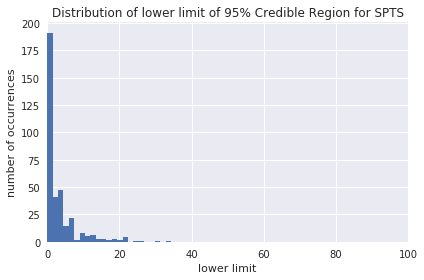
\includegraphics[scale=0.6]{SPTS_CR_analysis}
      \caption{Distribution of the left end point of the 95\% Credible Region for the SPTS network where the outcome was not within the Credible Region.}
      \label{fig:cranalysis}
    \end{figure}
    Thus, technically the observed outcomes are outside of the interval,
    but these lower limits are close enough to 0 for the practical purposes of TV planning.
    Removing the assumed right-censored data on this network, i.e.\ data in which $m_i^A = 0$,
    shows that 91.8\% of units are within the 95\% CR, a result consistent with the other networks.
    This information is useful as we will be able to forecast a range of possible outcomes for each
    unit of observation and be reasonably certain that the outcome will be within that range.

    \begin{table}[h!]
      \centering
        \begin{tabular}{lrrrr}
          & & \multicolumn{3}{c}{Credible Region $(1 - \alpha)\%$} \\
          network & level & $\alpha = 0.5$ & $\alpha = 0.05$ & $\alpha = 0.01$ \\
          \hline
          BCST & unit of observation & 0.465 & 0.922 & 0.966 \\
          ETMT & unit of observation & 0.48 & 0.91 & 0.95  \\
          SPTS & unit of observation & 0.416 & 0.765 & 0.799 \\
        \end{tabular}
      \caption{Proportion of units of observation that are within the listed Credible Region.}\label{tab:unitcr}
    \end{table}

  \end{section}

  \begin{section}{Aggregated Predictive Accuracy}

    Now that we have evaluated the accuracy of the forecasts on the units of observation,
    we want to evaluate the accuracy of the forecasts on aggregations of those units in the form of media plans.
    Under the model assumptions, the units of observation are exchangeable and given the model parameters,
    they are independently and identically distributed. Thus, we can assume that the
    forecasts under the model are independent and we can create the distribution
    of aggregated impressions through simple sums of the distribution of outcomes at the units of observation.

    We proceed as we did in the previous section by computing error metrics and Credible Regions
    of unit aggregations. Specifically, for each network, we quantile the units of observation
    in the hold-out set by the point forecasts of impression concentration for both models into 20 bins.
    We then compute the forecasted impressions for each quantile and compare to the actual impressions observed. For model $\mathcal{M}_0$
    this is merely the sum of the point estimates, but for model $\mathcal{M}$, this is the mean of the distribution of sums
    of impressions for the quantile.

    The graphical results of this analysis are shown in Figure \ref{fig:quantiledoutcomes}. From this
    graph we see that there is less dispersion in the forecasted versus actual values for model $\mathcal{M}$
    compared to model $\mathcal{M}_0$, especially for the SPTS network. However, graphs can sometime
    be misleading and so we analyze the resulting error metrics.

    \begin{figure}[!h]
      \centering
      \begin{subfigure}[b]{.75\textwidth}
        \centering
        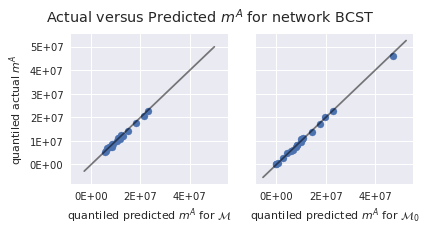
\includegraphics[scale=0.6]{BCST_quantiled}
      \end{subfigure}
      \begin{subfigure}[b]{.75\textwidth}
        \centering
        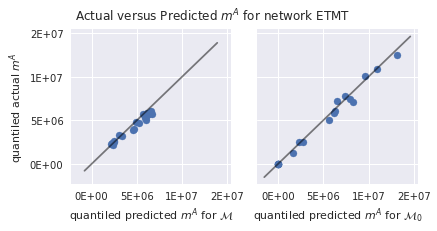
\includegraphics[scale=0.6]{ETMT_quantiled}
      \end{subfigure}
      \begin{subfigure}[b]{.75\textwidth}
        \centering
        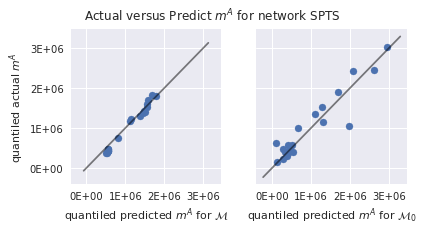
\includegraphics[scale=0.6]{SPTS_quantiled}
      \end{subfigure}
      \caption{Comparison of forecasts versus actuals for quantiled units of observation across the three networks
        for both models.}
      \label{fig:quantiledoutcomes}
    \end{figure}

    \begin{table}[h!]
      \centering
        \begin{tabular}{lrrrr}
          network & level & $\mathcal{M}_0$ MAE & $\mathcal{M}$ CRPS & $\mathcal{M}$ MAE \\
          \hline
          BCST & quantiled & 324034.14 & 277437.29 & 417797.60 \\
          ETMT & quantiled & 297512.52 & 311316.38 & 399648.10 \\
          SPTS & quantiled & 205096.15 & 75962.55 & 90668.35
        \end{tabular}
      \caption{Error metrics of the predicted data and the observed data in the hold-out set for the quantiled
        units of observation across the three networks.}\label{tab:quantileerror}
    \end{table}

    Tables \ref{tab:quantileerror} and \ref{tab:quantilecr} show that the same general story arises when looking at the
    quantiled units in aggregate as when looking at the units of observation; model $\mathcal{M}_0$ performs better
    than model $\mathcal{M}$ when only looking at the point forecasts, but model $\mathcal{M}$ outperforms
    when using the probabilistic forecasts, drastically so on the SPTS network.
    One notable exception is that the aggregation of units on ETMT do not seem to have the same performance
    in regard to error metrics and as the individual units themselves. This suggests that some
    model assumptions must not hold with this network and that the model needs to be re-evaluated.
    This is in-line with the previous model checks that showed misfit with this particular model.

    \begin{table}
      \centering
        \begin{tabular}{lrrrr}
          & & \multicolumn{3}{c}{Credible Region $(1 - \alpha)\%$} \\
          network & level & $\alpha = 0.5$ & $\alpha = 0.05$ & $\alpha = 0.01$ \\
          \hline
          BCST & quantiled & 0.45 & 0.95 & 1.0 \\
          ETMT & quantiled & 0.1 & 0.55  & 0.75 \\
          SPTS & quantiled & 0.4 & 0.65 & 0.65 \\
        \end{tabular}
      \caption{Proportion of quantiles that are within the listed Credible Region.}\label{tab:quantilecr}
    \end{table}

  \end{section}
\end{chapter}